\subsection{Properties of the binary classifier}

As shown in equation (\ref{rdef}), we summarize the result of a binary
classification using a single variable, $r \in [-1, ~+1]$, called the
{\it decision function}.  For a maximum
likelihood classification, we choose the threshold value for $r$, $r_0$,
that discriminates between the two classes:
\begin{equation}
c = \left \lbrace
\begin{array}{lr}
-1 & | r<r_0 \\
+1 & | r>r_0
\end{array}
\right .
\end{equation}
as $r_0 = 0$, but there is no reason why this should be so.  
In both \citet{Mills2009} and \citet{Mills2011}, we show how shifting this
border can be used to recalibrate an image derived from statistical
classification.

Since we are interested in deriving conditional probabilities from the 
multi-class classifier, 
we assume the decision function accurately estimates the
conditional probabilities as follows:
\begin{eqnarray}
	r_i(\vec x) & = & p_i(+1| \vec x) - p_i(-1| \vec x) \\
				       & = & \frac{p_i(+1, \vec x) - p_i(-1, \vec x)}{p_i(-1 , \vec x) + p_i(+1, \vec x)}
\end{eqnarray}

Note that because of the constraint in (\ref{first_constraint}) that
the conditional probabilities must sum to one,
we can express the decision function as both a difference in
conditional probabilities, $r$, as well as a ratio, $f$:
\begin{eqnarray}
	f & = & \frac{p(+1|\vec x)}{p(-1|\vec x)} \\
   & = & \frac{1 - p(-1|\vec x)}{p(-1|\vec x)}
\end{eqnarray}
Solving for $p(-1|\vec x)$ and equating the two produces the following:\
\begin{eqnarray}
	p(-1|\vec x) & = & \frac{1}{f+1} = \frac{1 - r_0}{2} \\
r_0 & = & \frac{f-1}{f+1} \\
f & = & \frac{1+r_0}{1-r_0}
\end{eqnarray}

Shifting the threshold can also be used to correct for the case in which we
are training the model using a set of samples whose class statistics
differ from those of the population.
Let $p(-1)$ and $p(+1)$ be the relative class numbers of the population while
$p^\prime(-1)$ and $p^\prime(+1)$ are the class numbers of the sample.
Typically, we want:
\begin{equation}
r=p(+1|\vec x)-p(-1|\vec x)=
\frac{p(+1)p(\vec x|+1)}{p(\vec x)}-\frac{p(-1)p(\vec x|-1)}{p(\vec x)} = 0
\end{equation}
or:
\begin{equation}
	\frac{p(\vec x|-1)}{p(\vec x|+1)}=\frac{p(+1)}{p(-1)}
\end{equation}
We want to find an $f$ such that the sample statistics are corrected to
the populations statistics:
\begin{equation}
f = \frac{p^\prime(+1)p(\vec x|+1)}{p^\prime(-1)p(\vec x|-1)}
=\frac{p^\prime(+1) p(-1)}{p^\prime(-1) p(+1)}
\end{equation}
or:
\begin{equation}
r_0=\frac{p^\prime(+1)p(-1) - p^\prime(-1) p(+1)}
	{p^\prime(+1)p(-1) + p^\prime(-1)p(+1)}
\end{equation}

\begin{figure}
\includegraphics[width=0.9\textwidth,angle=-90]{rhist.eps}
\caption{Cumulative distribution function (axes reversed) 
of the difference in conditional
probabilities, $r=p(+1|\vec x)-p(-1|\vec x)$
for the pair of sample classes described in \citet{Mills2011}.}
\label{rhist}
\end{figure}

\begin{figure}
\includegraphics[width=0.9\textwidth,angle=-90]{skillvsr0.eps}
\caption{Two skill scores, accuracy and uncertainty coefficient, as a function of
the decision threshold, $r_0$,
for the pair of sample classes described in \citet{Mills2011}.}
\label{skillvsr0}
\end{figure}

\begin{figure}
\includegraphics[width=0.9\textwidth,angle=-90]{sample_roc.eps}
Receiver operating characteristic (ROC) curve
for the pair of sample classes described in \citet{Mills2011}.
\label{sample_roc}
\end{figure}

In binary classification, the discrimination border can be shifted so as to
optimize any desired skill score.  Since only one parameter is being varied,
the optimization is a straightforward numerical procedure.  Any numerical
minimization technique, such as golden section search \citep{Press_etal1992},
that doesn't require derivatives (which will be discontinuous), can be used.

Figure \ref{rhist} shows the cumulative distribution,
$r$, $F(r)$ for the sample classes discussed in \citet{Mills2011}.  
From this, we can in theory
calculate any skill score for a binary classifier we desire, since:
\begin{eqnarray}
\frac{n_{TP}}{n} & = & \frac{1}{2}\int_{r_0}^{1} (r+1) 
		\frac{\mathrm d F}{\mathrm d r} \mathrm d r \\
\frac{n_{FP}}{n} & = & \frac{1}{2}\int_{r_0}^{1} (1-r) 
		\frac{\mathrm d F}{\mathrm d r} \mathrm d r \\
	& = & F(1) - F(r_0) - \frac{n_{TP}}{n} \\
\frac{n_{TN}}{n} & = & \frac{1}{2}\int_{-1}^{r_0} (1-r) 
		\frac{\mathrm d F}{\mathrm d r} \mathrm d r \\
\frac{n_{TP}}{n} & = & \frac{1}{2}\int_{-1}^{r_0} (r+1) 
		\frac{\mathrm d F}{\mathrm d r} \mathrm d r \\
	& = & F(r_0) - F(-1) - \frac{n_{TN}}{n} 
\end{eqnarray}
where $n_{TP}$, $n_{FP}$, $n_{TN}$, and $n_{FN}$ are the number of true positives
, false positive, true negative and false negatives, respectively, and $n$
is the total number of classes.
[integration by parts...]

The conditional probabilities are calculated based on the definitions of the
probability functions as described in \citet{Mills2011}.  For simple
accuracy, that is, fraction of correct predictions, the optimal decision
threshold should always lie close to zero, assuming the probabilities are
estimated accurately.  For the uncertainty coefficient, which measures the
number of bits of information contained in each prediction
\citep{Shannon, Press_etal1992, Mills2011}, changing the location of the
decision threshold can considerably improve skill scores.  In particular,
if one class is larger than the other, moving the decision border 
{\it closer} to it will typically improve the uncertainty coefficient.
These results are summarized in figure \ref{skillvsr0}.

Finally, the parameter, $r_0$, can also be used to construct 
the receiver operating characteristic (ROC) curve \citep{Jolliffe_Stephenson2003}.
The ROC curve for the pair of sample classes is shown in figure
\ref{sample_roc}.

Presumably, if the classes have been re-calibrated, then the associated 
conditional probabilities need to be transformed also.
Consider the following two transformations:
\begin{equation}
r^\prime = \left \lbrace
\begin{array}{lr}
\frac{r-r_0}{1-r_0} & r<r_0 \\
\frac{r_0-r}{r_0+1} & r>r_0
\end{array} \right \rbrace
\end{equation}
and:
\begin{equation}
r^\prime=\tanh \left (\tanh^{-1}(r)-\tanh^{-1}(r_0) \right ]
\end{equation}
with the second version being similar to what happens after setting the 
\verb/-r/ switch using \verb/class_borders/ in the {\it libagf} package.
Both these have the nice property both that transformed probabilities sum
to one and, if the original probability is one, then so are the transformed
probabilities:
\begin{equation}
p_i^\prime=1 \iff p_i=1
\label{ptop}
\end{equation}

Now consider a simple, linear transformation:
\begin{equation}
\vec p^\prime = A \vec p
\end{equation}
We wish to constrain the transformed probabilities, $\vec p^\prime$,
so that they sum to one as in (\ref{first_constraint}):
\begin{eqnarray}
\sum_i \sum_j a_{ij} p_j & = & 1 \\
\sum_i \sum_j a_{ij} p_j - \sum_j p_j & = & 0 \\
\sum_j p_j \left (\sum_i a_{ij} - 1 \right ) & = & 0
\end{eqnarray}
Thus all the columns of the transformation matrix must also sum to one:
\begin{equation}
\sum_i a_{ij} = 1
\end{equation}
In other words, the transformation matrix, $A$, is itself a conditional
probability.  If we wish to keep the constraint in (\ref{ptop}) then the only
solution is the identity matrix, $I$.


